\documentclass{beamer}
\graphicspath{ {figures/} }
\setbeamertemplate{page number in head/foot}[totalframenumber]
\usetheme{Marburg}
\newenvironment{system}%
{\left\lbrace\begin{array}{@{}l@{}}}%
{\end{array}\right.}

\beamersetuncovermixins{\opaqueness<1>{25}}{\opaqueness<2->{15}}
\begin{document}
\title{Mathematical Theory of Infectious Disease Epidemics}
\author{G. Hovhannisyan  A. Abrahamyan\\
M. Khachatryan}
\date{\today}


\begin{frame}
\titlepage
\end{frame}

\begin{frame}\frametitle{Table of contents}\tableofcontents
\end{frame}


\section{Introduction}
\begin{frame}\frametitle{Introduction}
    \begin{center}
        \textbf{Introduction}
    \end{center}
    \end{frame}

\begin{frame}\frametitle{Introduction}
\begin{center}
    \begin{columns}
        \begin{column}{5cm}
        \begin{itemize}
        \item Model Diseases
        \item Predict Their Future Behavior
        \item Managing Their Spread
        \end{itemize}
        \end{column}
        \begin{column}{5cm}
        \begin{figure}
            \caption{Example of SIR}
	        \centering
	        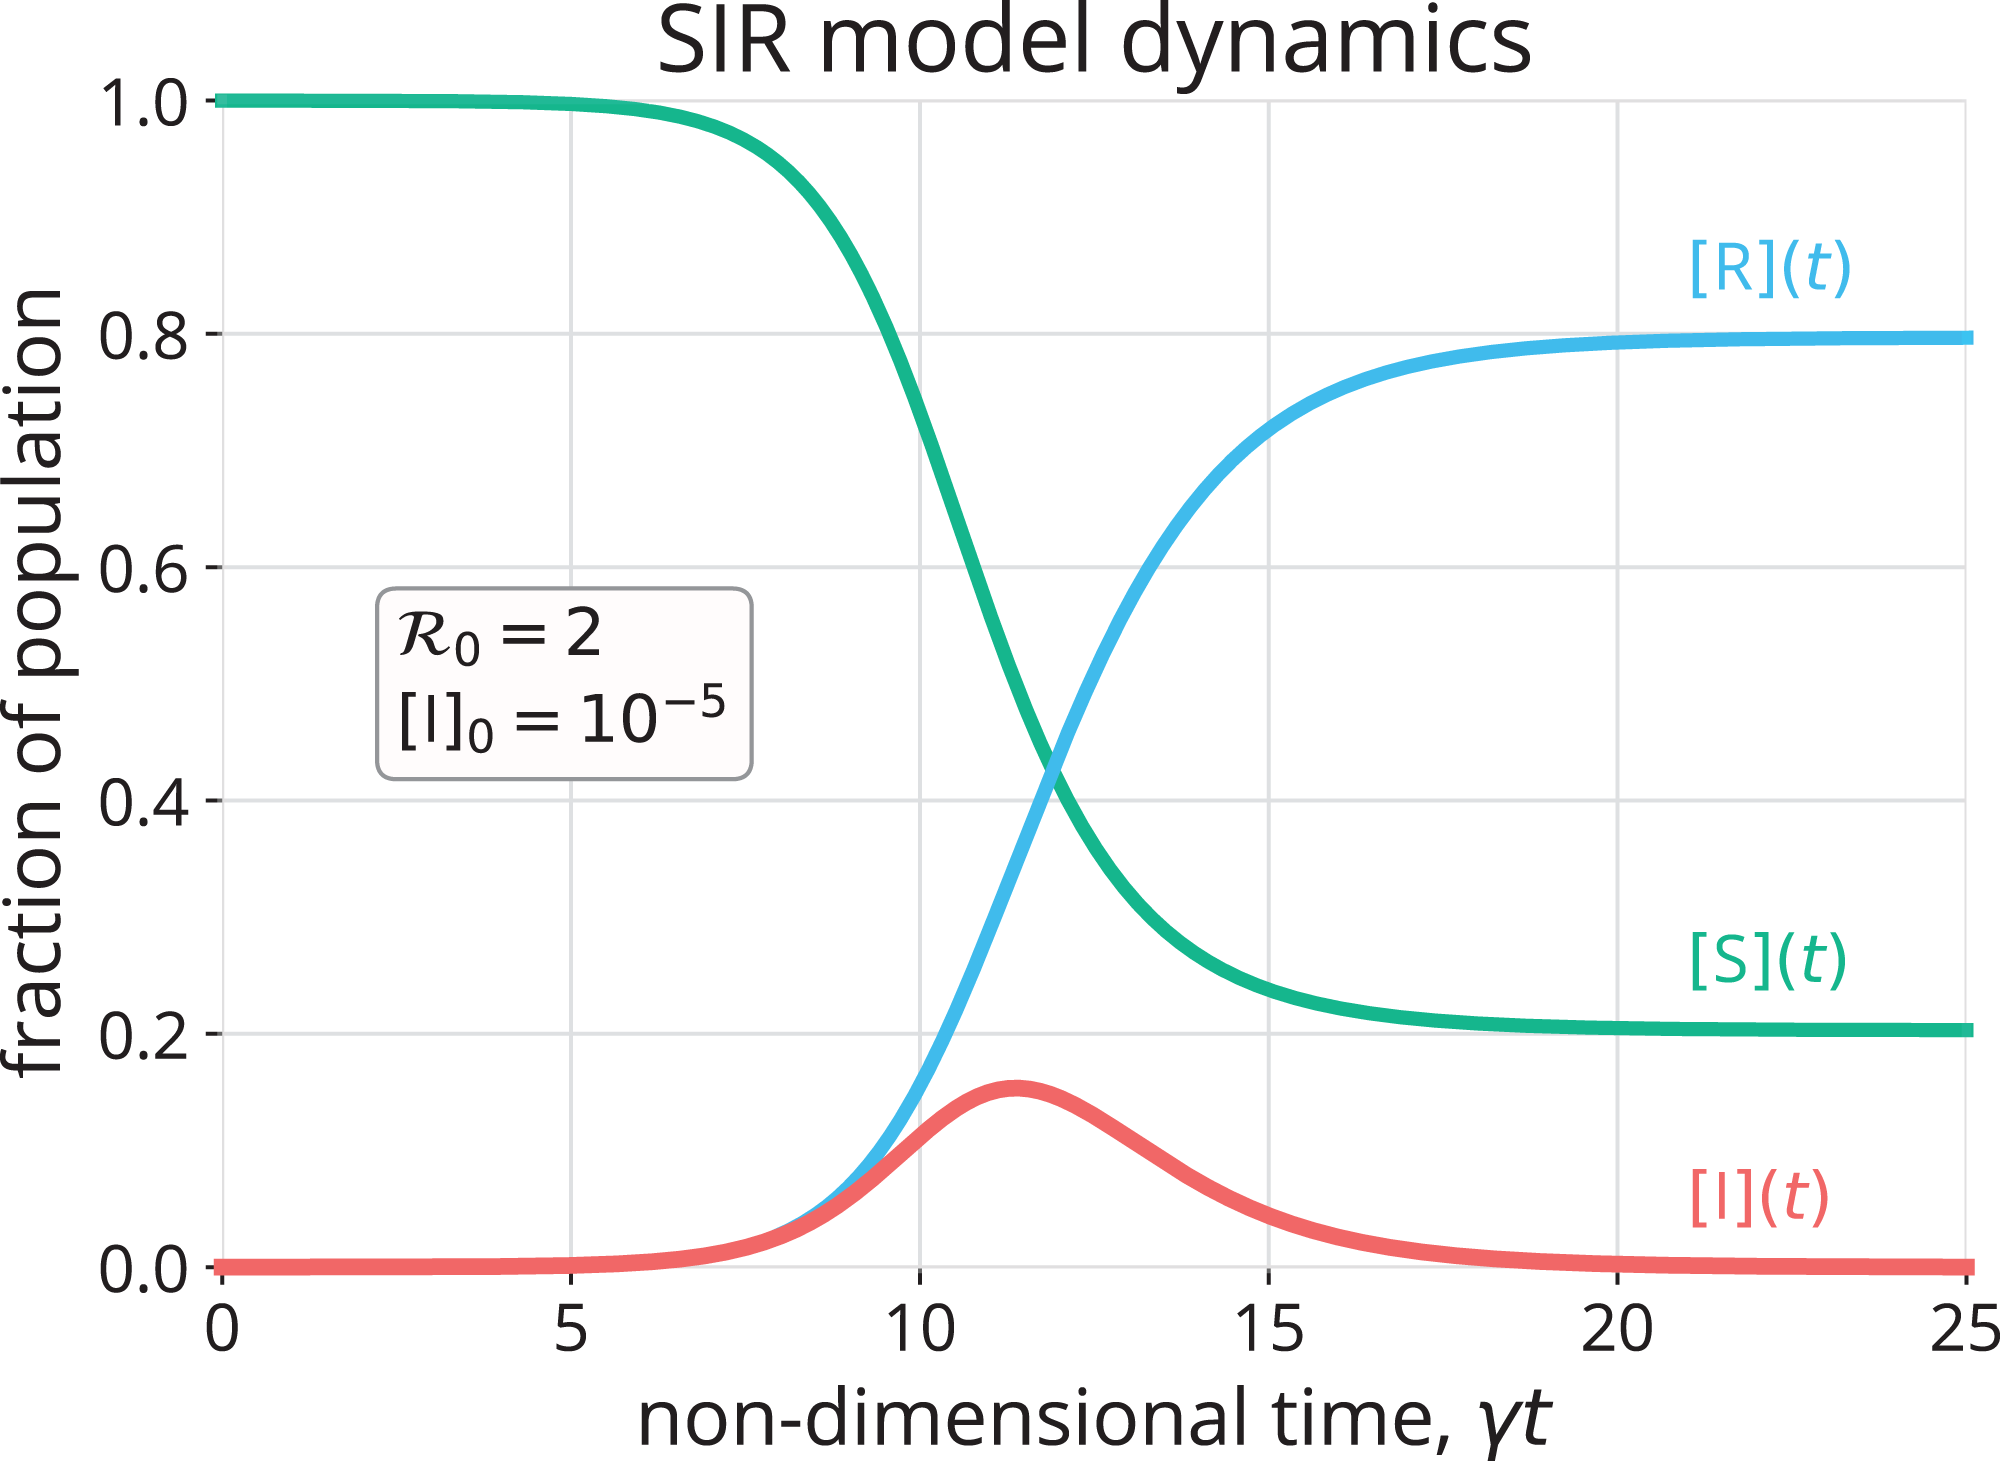
\includegraphics[width=5cm]{Figure1.png}
        \end{figure}
        \end{column}
        \end{columns}
\end{center}
\end{frame}

\section{Mathematical Formulation}
\begin{frame}\frametitle{Mathematical Formulation}
\begin{center}
    \textbf{Mathematical Formulation}
\end{center}
\end{frame}


\begin{frame}\frametitle{Mathematical Formulation}
\begin{itemize}
\item Types of Variables
\item Important Assumptions
\end{itemize}
\end{frame}

\subsection{Types of Variables}
\begin{frame}\frametitle{Independent and Dependent Variables}
    The only dependent variable is $t$(time) measured in days.\\
    \vspace{0.15in}
    The first set of dependent variables are functions of time, which count people in each group.
    $$S(t)\text{ is the number of \textit{susceptible} individuals at given time,}$$
    $$I(t)\text{ is the number of \textit{infected} individuals at give time,}$$
    $$R(t)\text{ is the number of \textit{recovered} individuals at give time.}$$
\end{frame}

\begin{frame}\frametitle{Independent and Dependent Variables}
The second set of dependent variables represents the \textit{fraction} of the total population in
each of the three categories. So, if $N$ is the total population we have:
    $$s(t) = \frac{S(t)}{N}\text{ the \textit{susceptible fraction} of the population,}$$
    $$i(t) = \frac{I(t)}{N}\text{the \textit{infected fraction} of the population, and}$$
    $$r(t) = \frac{R(t)}{N}\text{the \textit{recovered fraction} of the population.}$$
\end{frame}

\begin{frame}[t]\frametitle{Importnat Assumptions}
These assumptions inform the derivatives of our dependent variables.
    \begin{itemize}
        \item $\frac{\partial{s}}{\partial{t}}=-\beta s(t)i(t)$
        \item $\frac{\partial{r}}{\partial{t}}=\gamma i(t)$
    \end{itemize}
\begin{align}
    \frac{\partial{s}}{\partial{t}}&=-\beta s(t)i(t)\\
    \frac{\partial{r}}{\partial{t}}&=\gamma i(t)
\end{align}

As the sum of \textit{susceptable}, \textit{infected} and \textit{recovered} people gives the whole population, it means that
\begin{align}
    \frac{\partial{s}}{\partial{t}}+\frac{\partial{i}}{\partial{t}}+\frac{\partial{r}}{\partial{t}}=0
\end{align}

To get the differential equation for infecteds it is enough to plug equations (1) and (2)
into equation (3). The result will be:
    \begin{align}
        \frac{\partial{i}}{\partial{t}}=-\beta s(t)i(t)-\gamma i(t)
    \end{align}
\end{frame}

\begin{frame}\frametitle{Important Assumptions}
Combining all three equations will give the following system of differential equations:
\begin{equation*}
    \begin{system}
        \frac{\partial{s}}{\partial{t}}=-\beta s(t)i(t)\\
        \\
        \frac{\partial{i}}{\partial{t}}=-\beta s(t)i(t)-\gamma i(t)\\
        \\
        \frac{\partial{r}}{\partial{t}}=\gamma i(t)
    \end{system}
\end{equation*}
\end{frame}

\section{Analytical Solution}
\begin{frame}\frametitle{Analytical Solution}
\begin{center}
    \textbf{Analytical Solution}
\end{center}
\end{frame}


\begin{frame}\frametitle{Analytical Solution}
\begin{equation*}
    \begin{system}
        x^{\prime} = -\beta x  y 
		\\
		y^{\prime} = \beta x  y - \gamma y 
		\\
		z^{\prime} = \gamma z 
		\\
		x + y + z = N
		\\
		x_0 = N_1, y_0 = N_2, z_0 = N_3
    \end{system}
\end{equation*}
Step 1) Differentiating $x$ with respect to time $t$, and substituting $y^{\prime}$.
\begin{equation*} 
	\begin{split}
		x^{\prime\prime} =
		-\beta\left( x^{\prime}\left(\frac{-x^{\prime}}{\beta x}\right) + x y^{\prime}\right)
		 & \implies \frac{-x^{\prime\prime}}{\beta} = \frac{-(x^{\prime})^{2}}{\beta x} + x y^{\prime}                             \\
		 & \implies x y^{\prime} = \frac{-x^{\prime\prime}}{\beta} + \frac{-(x^{\prime})^{2}}{\beta x}                             \\
		 & \implies y^{\prime} =  \frac{-1}{\beta}\left(\frac{-x^{\prime\prime}}{x} - \left(\frac{x^{\prime}}{x}\right)^{2}\right)
	\end{split}
\end{equation*}
\end{frame}

\begin{frame}\frametitle{Analytical Solution}
Step 2) Next we insert $y = \frac{-x^{\prime}}{\beta x}$ into $y^{\prime}$ and equate it to \\Step (1)
\begin{equation*} 
	\begin{split}
		-x^{\prime} + \frac{\gamma x^{\prime}}{\beta x} =
		\frac{-1}{\beta}\left(\frac{-x^{\prime\prime}}{x} - \left(\frac{x^{\prime}}{x}\right)^{2}\right)\\
		\implies \beta x^{\prime} - \frac{\gamma x^{\prime}}{x} = \frac{x^{\prime\prime}}{x} - \left(\frac{x^{\prime}}{x}\right)^{2}    \\
		\implies \frac{x^{\prime\prime}}{x} - \left(\frac{x^{\prime}}{x}\right)^{2} + \frac{\gamma x^{\prime}}{x} - \beta x^{\prime}= 0
	\end{split}
\end{equation*}
Step 3) We also have that $y = \frac{-x^{\prime}}{\beta x}$ and $y = \frac{z^{\prime}}{\gamma}$.
Equating them we get
\begin{equation*}
	\frac{-x^{\prime}}{\beta x} = \frac{z^{\prime}}{\gamma}
	\implies z^{\prime} = -\frac{\gamma}{\beta}\left(\frac{x^{\prime}}{x}\right)
\end{equation*}
\end{frame}

\begin{frame}\frametitle{Analytical Solution}
Step 4) Next we integrate Step (3)
\begin{equation*} 
	\begin{split}
		c_{1} + z = -\frac{\gamma}{\beta} \int \frac{x^{\prime}}{x} \,dt
		 & \implies c_{1} + z = -\frac{\gamma}{\beta}\left(\ln(x) + c_{2}\right)                                       \\
		 & \implies \ln(x) = -\frac{\beta c_{1}}{\gamma} -\frac{\beta z}{\gamma} - c_{2}                               \\
		 & \implies x = e^{-\frac{\beta z}{\gamma}} \cdot e^{-\frac{\beta c_{1}}{\gamma} - c_{2}}                      \\
		 & \implies x = x_{0}e^{-\frac{\beta z}{\gamma}}  \hspace{\parindent}  
	\end{split}
\end{equation*}
Where $x_{0}$ is an integration constant.
\end{frame}

\begin{frame}\frametitle{Analytical Solution}
    Step 5) From Step(4) we get that 
    \begin{equation*} 
        x^{\prime} = -\frac{x_{0}\beta}{\gamma} z^{\prime} e^{-\frac{\beta z}{\gamma}}
    \end{equation*}
    Step 6) Instead of integrating we differentiate Step (3) and get
    \begin{equation*}
        z^{\prime\prime} = -\frac{\gamma}{\beta}\left(\frac{x^{\prime\prime}}{x} - \left(\frac{x^{\prime}}{x}\right)^{2} \right)
    \end{equation*}
    Step 7) Finally if we combine Step(6), Step(5) and Step(3) into Step(2) we get
    \begin{equation*}
        z^{\prime\prime} = x_{0} \beta z^{\prime} e^{-\frac{\beta z}{\gamma}} - \gamma z^{\prime}
    \end{equation*}
\end{frame}

\begin{frame}\frametitle{Analytical Solution}
    All the other steps can be found in the paper in Appendix B, but eventually we get the parametric form
    \begin{align*}
        x &= x_0u,\\
        y &= \frac{\gamma}{\beta}\ln u - x_0u - \frac{C_1}{\beta},\\
        z &= -\frac{\gamma}{\beta}\ln u
    \end{align*}
Where $u_0 = e^{-\frac{\beta}{\gamma}N_3}$, $C_1 = -\beta N$.\\
And the relation between $u$ and $t$ being as follows
\begin{equation*} 
	t = \int_{u_0}^{u} \frac{du}{u(C_1-\gamma \ln u + x_0\beta u)}
\end{equation*}
\end{frame}
\begin{frame}\frametitle{Analytical Solution}
    \begin{figure}
        \caption{Graphical Examples of the Analytical Solution}
        \centering
        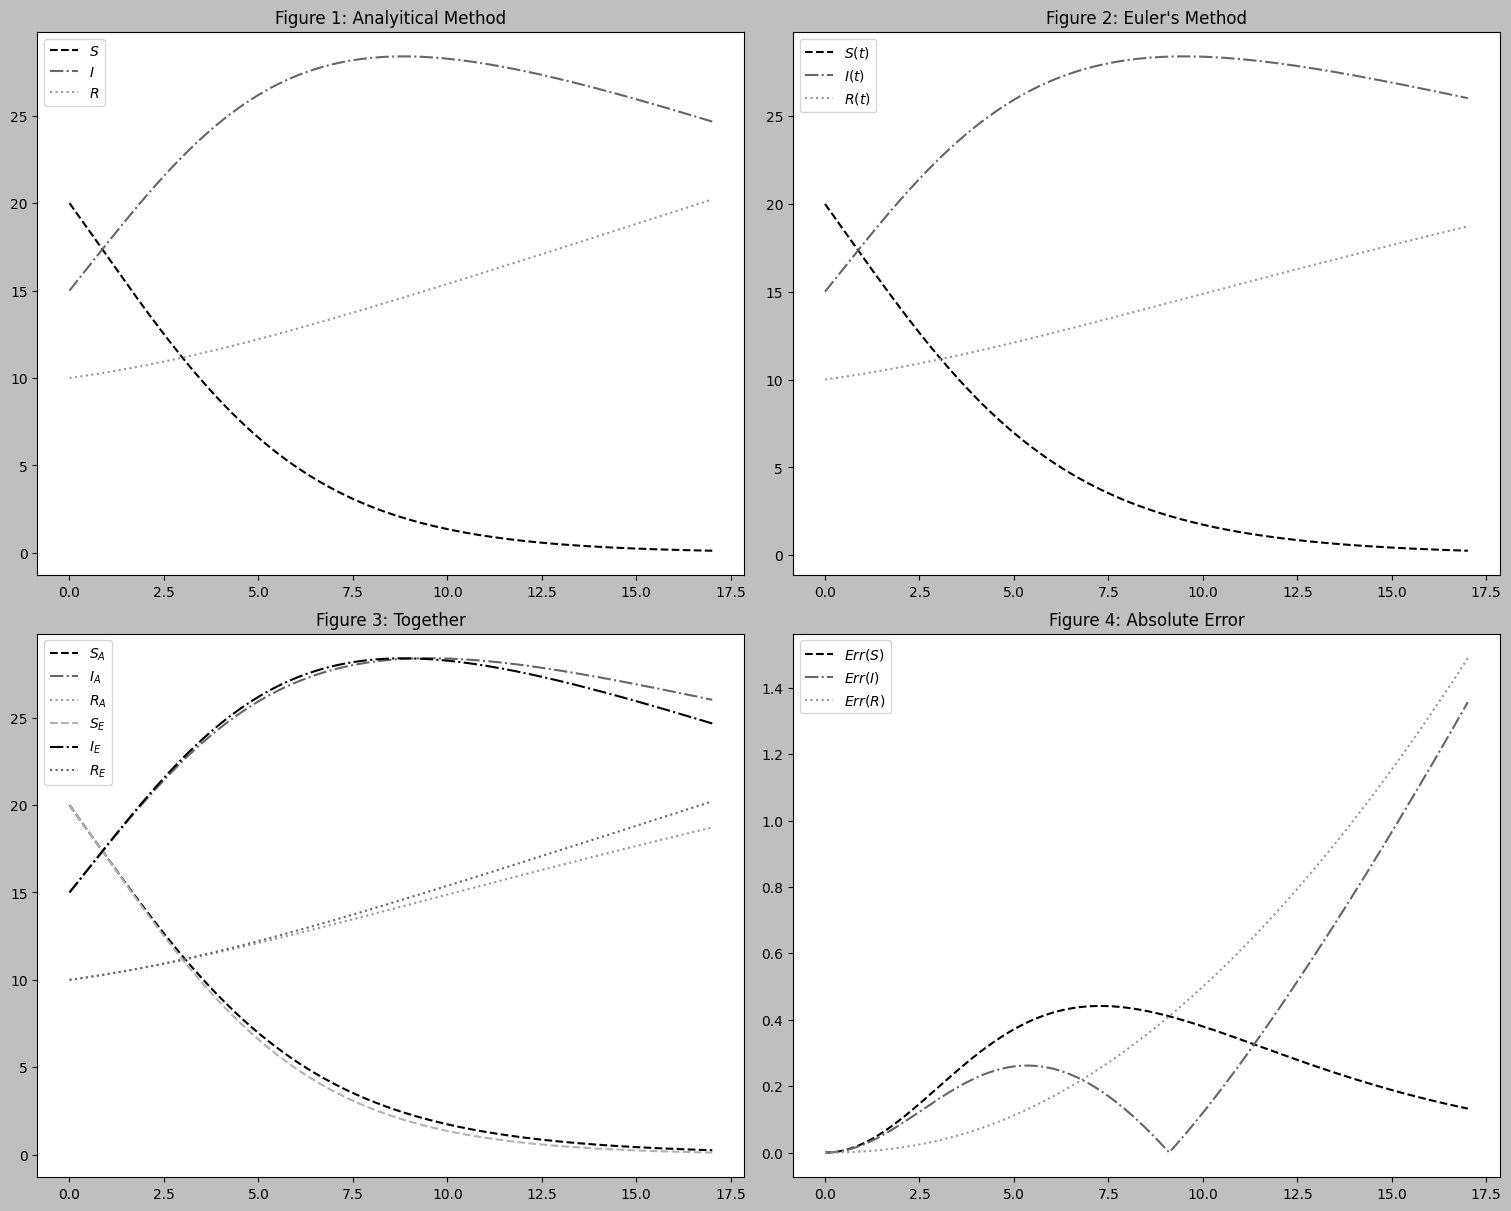
\includegraphics[width=8cm]{Figure_Analitical.png}
    \end{figure}

    Plotted Using Values$\quad$ $N_1=20, \quad N_2=15, \quad N_3=10, \quad \beta = 0.01, \quad \gamma = 0.02$
\end{frame}



\section{Numerical Methods for Solving the SIR}
\subsection{blocs}
\begin{frame}\frametitle{blocs}


\begin{exampleblock}{title of the bloc}
bloc text
\end{exampleblock}


\begin{alertblock}{title of the bloc}
bloc text
\end{alertblock}
\end{frame}


\section{Simulation Results on Real-World Data}
\subsection{split screen}

\begin{frame}\frametitle{splitting screen}
\begin{columns}
\begin{column}{5cm}
\begin{itemize}
\item Beamer
\item Beamer Class
\item Beamer Class Latex
\end{itemize}
\end{column}
\begin{column}{5cm}
\begin{tabular}{|c|c|}
\hline
\textbf{Instructor} & \textbf{Title} \\
\hline
Sascha Frank &  \LaTeX \ Course 1 \\
\hline
Sascha Frank &  Course serial  \\
\hline
\end{tabular}
\end{column}
\end{columns}
\end{frame}

\subsection{Pictures}
\begin{frame}\frametitle{pictures in latex beamer class}
\begin{figure}
\caption{show an example picture}
\end{figure}
\end{frame}

\subsection{joining picture and lists}

\begin{frame}
\frametitle{pictures and lists in beamer class}
\begin{columns}
\begin{column}{5cm}
\begin{itemize}
\item<1-> subject 1
\item<3-> subject 2
\item<5-> subject 3
\end{itemize}
\vspace{3cm}
\end{column}
\begin{column}{5cm}
\begin{overprint}
\end{overprint}
\end{column}
\end{columns}
\end{frame}


\subsection{pictures which need more space}
\begin{frame}[plain]
\frametitle{plain, or a way to get more space}
\begin{figure}
\caption{show an example picture}
\end{figure}
\end{frame}



\end{document}